Nous allons d\'eterminer la matrice d'adjacence du graphe de corr\'elation \`a partir des valeurs de $M_c$.
\newline 
Soit $s = \{ 0.1, \cdots, 0.9\}$, une valeur de seuil choisie.
Nous construisons la matrice $M_s$  selon les r\`egles suivantes : 
\begin{itemize}
\item Si $M_c[i,j] \ge s$ alors $M_s[i,j] = 1$.
\item Si $M_c[i,j] < s$ alors $M_s[i,j] = 0$.
\end{itemize}
La matrice $M_s$ est la matrice d'adjacence du graphe $G_s$  dit {\em graphe de corr\'elation}. Ces cases peuvent contenir des cases erron\'ees. Ces cases erron\'ees proviennent de la s\'election du seuil $s$ et de la g\'en\'eration de valeurs de corr\'elation pour les cases \`a $0$ et \`a $1$ du line-graphe $LG$. En effet ,
\begin{itemize}
	\item Si $M_s [i,j] = M_{LG} [i,j] = 0$ alors $M_{s} [i,j]$ est dit {\em vrai n\'egatif}. 
	\item Si $M_s [i,j] = M_{LG} [i,j] = 1$ alors $M_{s} [i,j]$ est dit {\em vrai positif}. 
	\item Si $M_s [i,j] = 0$ et $M_{LG} [i,j] = 1$ alors $M_{s} [i,j]$ est dit {\em faux n\'egatif}.
	\item Si $M_s [i,j] = 1$ et $M_{LG} [i,j] = 0$ alors $M_{s} [i,j]$ est dit {\em faux positif}.
\end{itemize}
Un exemple de distributions des cases erron\'ees selon les valeurs de seuils est pr\'esent\'e dans la figure \ref{distrib_relationAdjacence_seuils}. 
%---------------- distributionsCases01avecCoefficientAsymetries ------------------
\begin{figure}[htb!] 
\centering
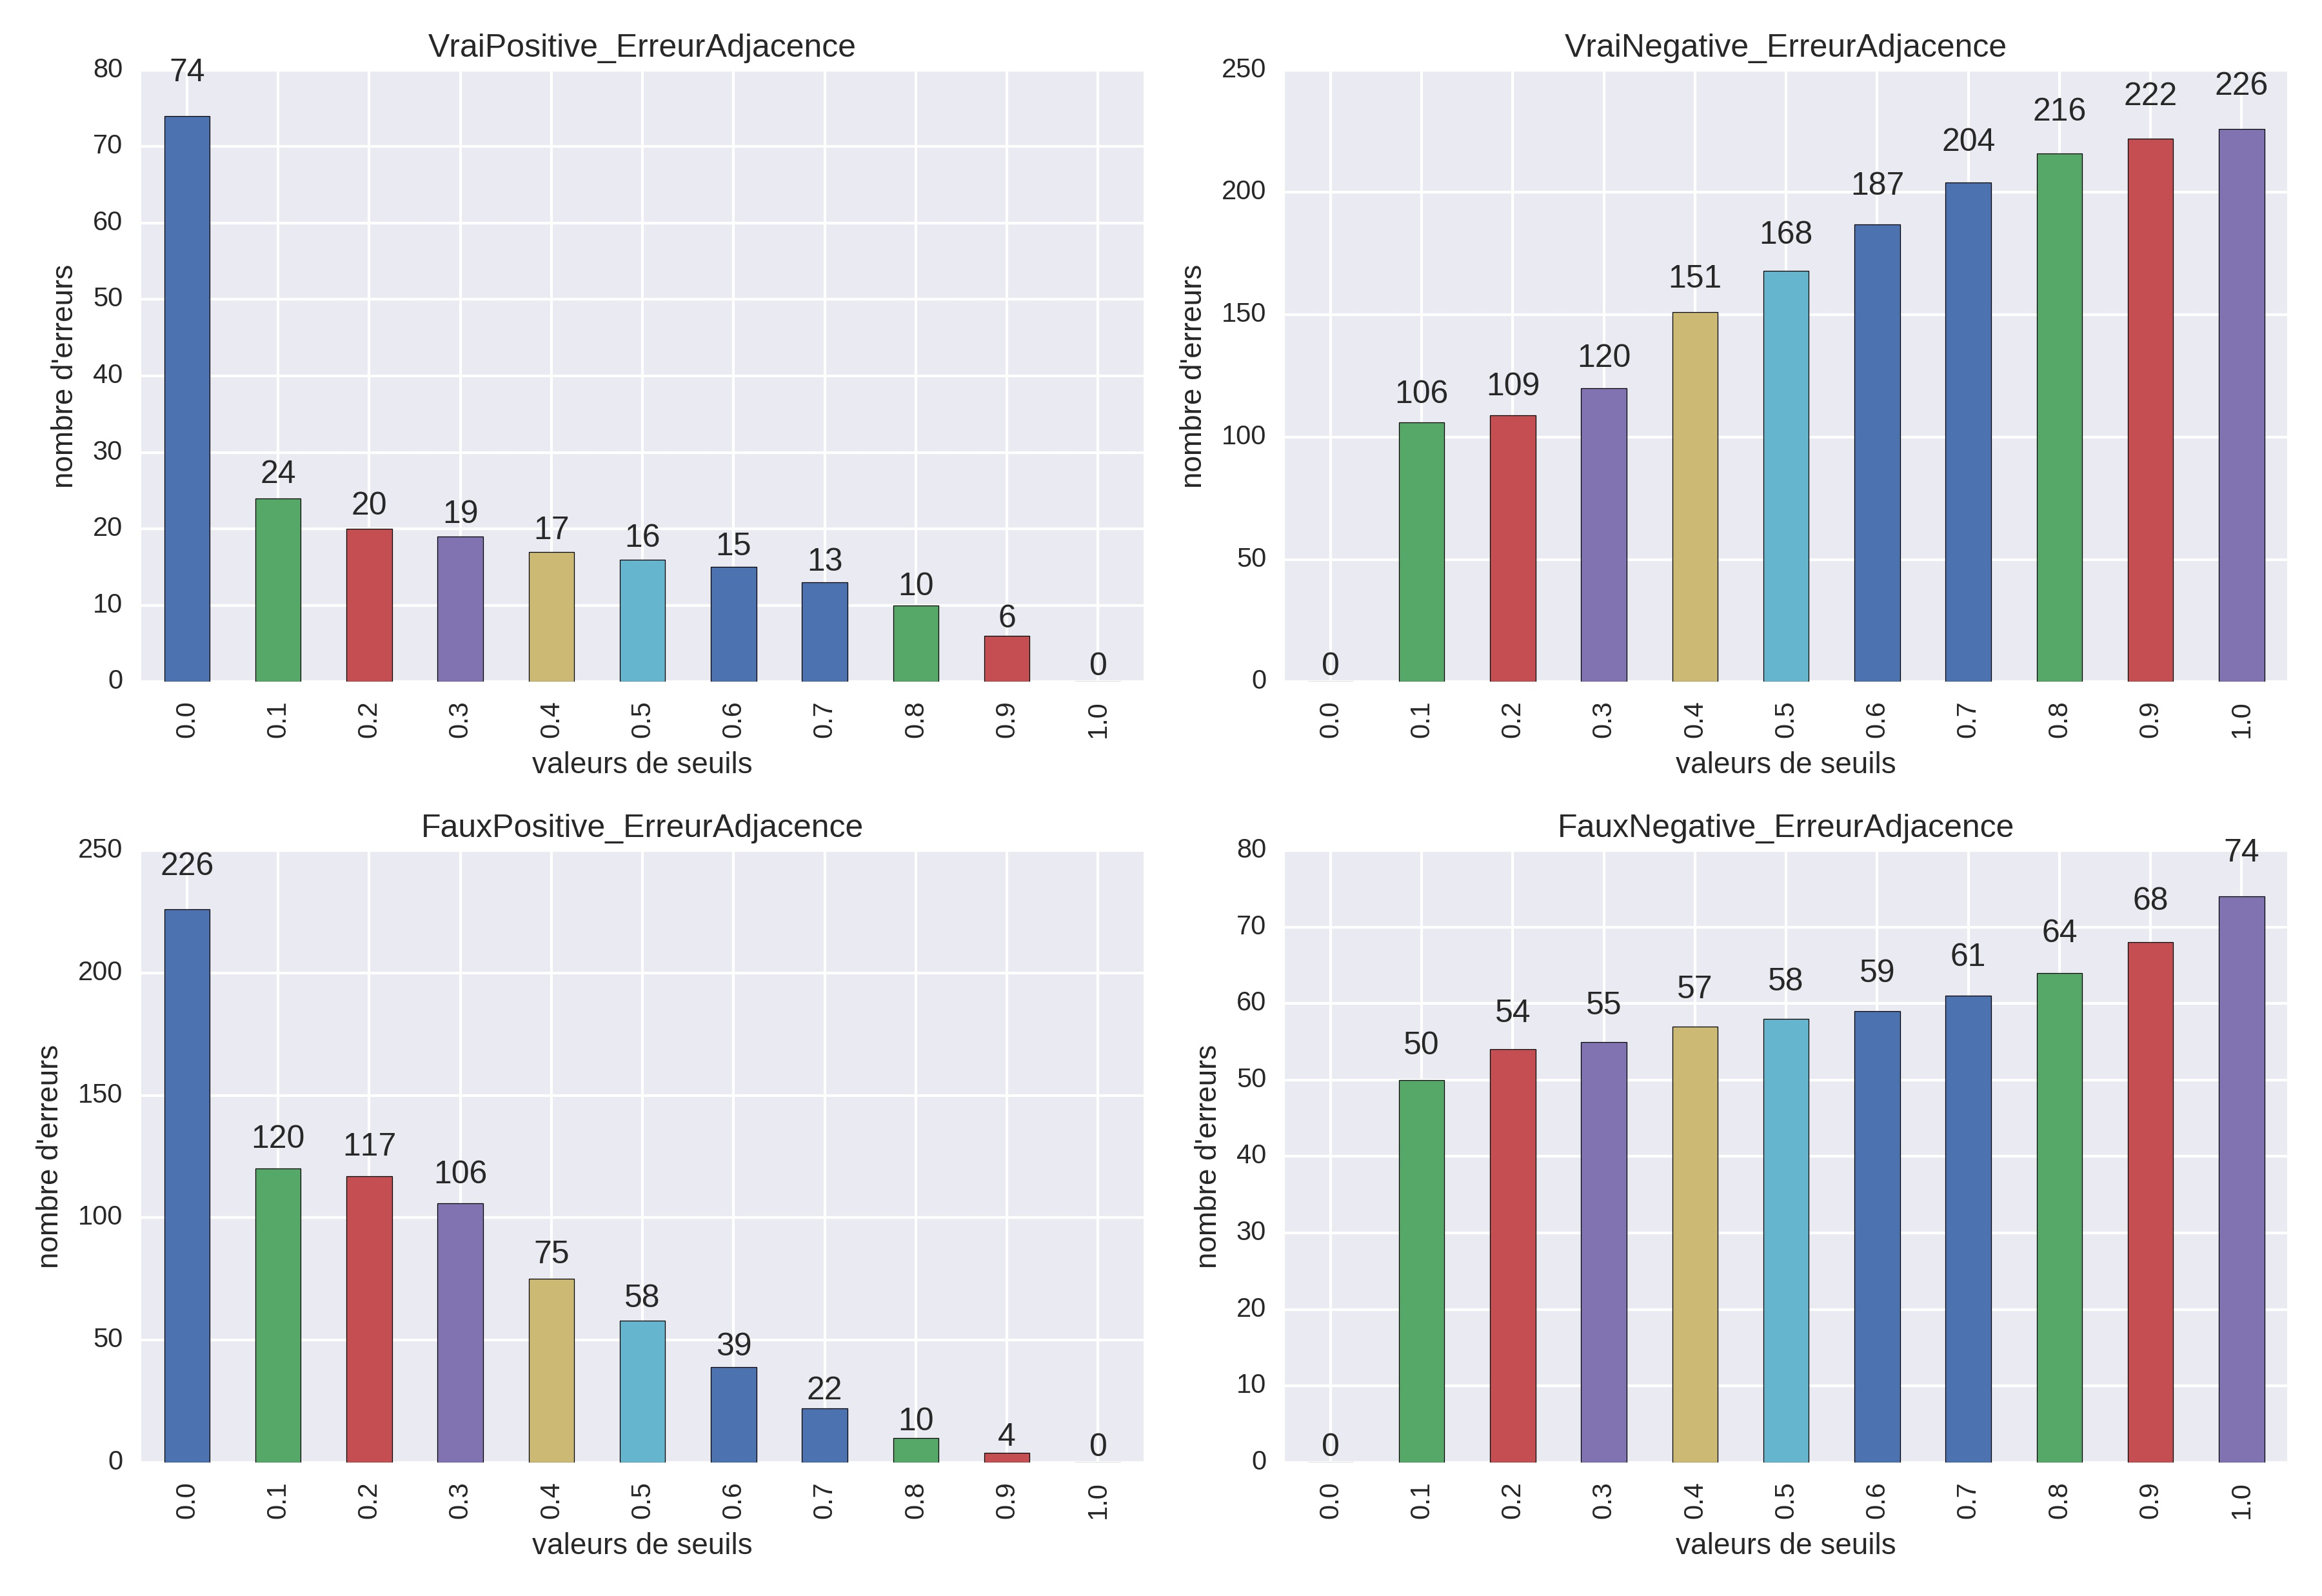
\includegraphics[width=500pt,height=250pt]{distrib_relationAdjacence_seuils.jpeg}
\caption{ Distribution des valeurs de corr\'elation sur un graphe g\'en\'er\'e de $30$ sommets et de degr\'e maximal de $5$.
.}
\label{distrib_relationAdjacence_seuils} 
\end{figure}
% \FloatBarrier
%---------------- distributionsCases01avecCoefficientAsymetries ------------------
Par exemple,  le graphe de corr\'elation $G_s$ contient 
$17$ cases {\em vrais positives}, 
$151$ cases {\em vrais n\'egatives}, 
$75$ cases {\em fausses positives} et 
$57$ cases {\em fausses n\'egatives} pour un seuil $s=0.4$.
